% Vectorized (AVX-2) two-level bin search over 64 histogram bin boundaries,
% Avx2UpperBoundIndex64 in training.cc: coarse8[g] = thr64[(g+1)*8-1], K = popcnt.
% Companion panel: binary_search_illustration.tex
% Palette matches figures/method/double_sparsity_illustration.pdf.
\definecolor{figblue}{HTML}{2A6AB5}
\definecolor{figbluefill}{HTML}{4A90D9}
\definecolor{figgreen}{HTML}{3D8B5E}
\definecolor{figgreenfill}{HTML}{B8E6C8}
\definecolor{figamber}{HTML}{FDE68A}
\definecolor{figamberdark}{HTML}{B8860B}
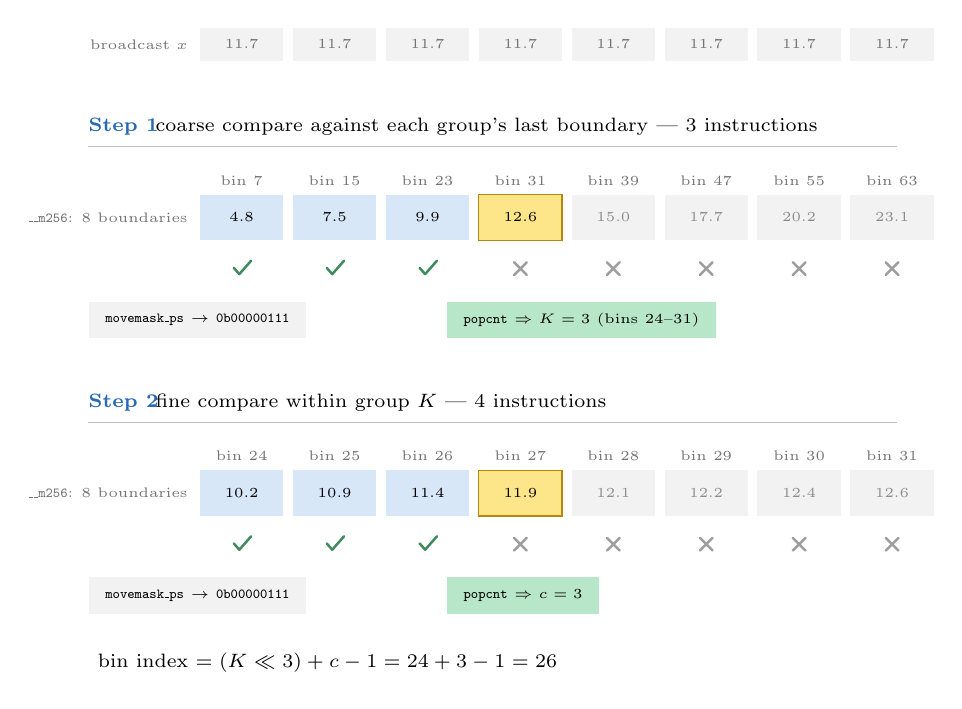
\begin{tikzpicture}[
  x=1cm, y=1cm, font=\scriptsize,
  lane/.style={rectangle, minimum width=1.06cm, minimum height=0.58cm,
               inner sep=0pt, align=center, font=\tiny},
  pass/.style={lane, fill=figbluefill!22},
  stop/.style={lane, fill=figamber, draw=figamberdark, line width=0.5pt},
  off/.style={lane, fill=black!5, text=black!45},
  bcast/.style={lane, minimum height=0.42cm, fill=black!5, text=black!55},
  hdr/.style={font=\scriptsize\bfseries, text=figblue, anchor=west, inner sep=0pt},
  sub/.style={font=\scriptsize, anchor=west, inner sep=0pt},
  rowlab/.style={font=\tiny, text=black!55, anchor=east, inner sep=0pt},
  tag/.style={font=\tiny, text=black!55, anchor=south, inner sep=1.5pt},
  bar/.style={rectangle, fill=black!5, minimum height=0.46cm, inner xsep=6pt,
              inner ysep=0pt, font=\tiny, anchor=west},
  res/.style={rectangle, fill=figgreenfill, minimum height=0.46cm, inner xsep=6pt,
              inner ysep=0pt, font=\tiny, anchor=west},
  yes/.pic={\draw[figgreen, line width=0.9pt, line cap=round, line join=round]
              (-0.10,0.01) -- (-0.03,-0.07) -- (0.12,0.10);},
  no/.pic={\draw[black!38, line width=0.9pt, line cap=round]
              (-0.08,-0.08) -- (0.08,0.08) (-0.08,0.08) -- (0.08,-0.08);}]

  \def\p{1.18}   % lane pitch
  \def\W{8.32}   % right edge of the lane strip

  % ---- broadcast -------------------------------------------------------
  \node[rowlab] at (-0.68,0) {broadcast $x$};
  \foreach \i in {0,...,7} { \node[bcast] at (\i*\p,0) {11.7}; }

  % ---- step 1: coarse ---------------------------------------------------
  \node[hdr] at (-1.95,-1.05) {Step 1};
  \node[sub] at (-1.10,-1.05)
    {coarse compare against each group's last boundary \textnormal{--- 3 instructions}};
  \draw[black!25, line width=0.4pt] (-1.95,-1.30) -- (\W,-1.30);

  \foreach \i/\b in {0/7, 1/15, 2/23, 3/31, 4/39, 5/47, 6/55, 7/63} {
    \node[tag] at (\i*\p,-1.85) {bin \b};
  }
  \foreach \i/\v in {0/4.8, 1/7.5, 2/9.9} {
    \node[pass] at (\i*\p,-2.20) {\v};
    \pic at (\i*\p,-2.85) {yes};
  }
  \node[stop] at (3*\p,-2.20) {12.6};
  \pic at (3*\p,-2.85) {no};
  \foreach \i/\v in {4/15.0, 5/17.7, 6/20.2, 7/23.1} {
    \node[off] at (\i*\p,-2.20) {\v};
    \pic at (\i*\p,-2.85) {no};
  }
  \node[rowlab] at (-0.68,-2.20) {\texttt{\_\_m256}: 8 boundaries};

  \node[bar] at (-1.95,-3.50) {\texttt{movemask\_ps} $\rightarrow$ \texttt{0b00000111}};
  \node[res] at (2.60,-3.50) {\texttt{popcnt} $\Rightarrow K=3$ (bins 24--31)};

  % ---- step 2: fine -----------------------------------------------------
  \node[hdr] at (-1.95,-4.55) {Step 2};
  \node[sub] at (-1.10,-4.55)
    {fine compare within group $K$ \textnormal{--- 4 instructions}};
  \draw[black!25, line width=0.4pt] (-1.95,-4.80) -- (\W,-4.80);

  \foreach \i/\b in {0/24, 1/25, 2/26, 3/27, 4/28, 5/29, 6/30, 7/31} {
    \node[tag] at (\i*\p,-5.35) {bin \b};
  }
  \foreach \i/\v in {0/10.2, 1/10.9, 2/11.4} {
    \node[pass] at (\i*\p,-5.70) {\v};
    \pic at (\i*\p,-6.35) {yes};
  }
  \node[stop] at (3*\p,-5.70) {11.9};
  \pic at (3*\p,-6.35) {no};
  \foreach \i/\v in {4/12.1, 5/12.2, 6/12.4, 7/12.6} {
    \node[off] at (\i*\p,-5.70) {\v};
    \pic at (\i*\p,-6.35) {no};
  }
  \node[rowlab] at (-0.68,-5.70) {\texttt{\_\_m256}: 8 boundaries};

  \node[bar] at (-1.95,-7.00) {\texttt{movemask\_ps} $\rightarrow$ \texttt{0b00000111}};
  \node[res] at (2.60,-7.00) {\texttt{popcnt} $\Rightarrow c=3$};

  \node[anchor=west, font=\scriptsize] at (-1.95,-7.85)
    {bin index $=(K\ll 3)+c-1=24+3-1=26$};
\end{tikzpicture}
